% =============================================================
% Annexure H: Full Hyperparameter Grid Results
% =============================================================
\section{Full Hyperparameter Grid Results}
\label{annexure:hyperparameters}

% -------------------------------------------------------------
\subsection{Five-Phase Sequential Comparison}
\label{annexure:five_phase}

Hyperparameters were selected through a five-phase sequential comparison procedure. In each phase, one hyperparameter was varied while all others were held at their current best values. The phases proceeded in the following order:

\begin{enumerate}
    \item Activation function (CELU, GELU, Tanh), with fixed lr${}=0.001$, batch size${}=256$, Adam.
    \item Learning rate ($0.01, 0.001, 0.0005, 0.0001$), with fixed best activation, batch size${}=256$, Adam.
    \item Batch size ($64, 128, 256, 512$), with fixed best activation and learning rate, Adam.
    \item Optimiser (Adam vs NAdam), with all previous best values fixed.
    \item Momentum $\beta_1$ ($0.90, 0.95, 0.99$) with $\beta_2 = 0.999$ fixed, using the best optimiser.
\end{enumerate}

Each configuration was trained with early stopping (patience of 10 validation checks at 5-epoch intervals) up to a maximum of 100 epochs. Table~\ref{tab:hyper_full} reports the full results.

\begin{table}[htbp]
\centering
\caption{Full five-phase hyperparameter comparison results.}
\label{tab:hyper_full}
\footnotesize
\begin{tabular}{llrrr}
\toprule
\textbf{Phase} & \textbf{Configuration} & \textbf{Best Epoch} & \textbf{Val $R^2$} & \textbf{Time (s)} \\
\midrule
\multirow{3}{*}{Phase 1: Activation}
  & CELU  & 100 & 0.995682 & 556.7 \\
  & GELU  &  25 & 0.995636 & 313.8 \\
  & Tanh  & 100 & 0.995532 & 565.9 \\
\midrule
\multirow{4}{*}{Phase 2: Learning Rate}
  & 0.01   &  10 & 0.995453 & 222.9 \\
  & 0.001  & 100 & 0.995682 & 558.1 \\
  & 0.0005 & 100 & 0.995692 & 563.8 \\
  & 0.0001 & 100 & 0.995686 & 556.0 \\
\midrule
\multirow{4}{*}{Phase 3: Batch Size}
  & 64  &  75 & 0.995678 & 1441.8 \\
  & 128 &  30 & 0.995669 &  491.9 \\
  & 256 & 100 & 0.995692 &  580.3 \\
  & 512 & 160 & 0.995685 &  487.3 \\
\midrule
\multirow{2}{*}{Phase 4: Optimiser}
  & Adam  & 100 & 0.995692 & 562.7 \\
  & NAdam &  85 & 0.995693 & 582.5 \\
\midrule
\multirow{3}{*}{Phase 5: Momentum}
  & $\beta_1=0.90$ & 85 & 0.995693 & 586.6 \\
  & $\beta_1=0.95$ & 40 & 0.995690 & 427.8 \\
  & $\beta_1=0.99$ & 95 & 0.995685 & 621.8 \\
\bottomrule
\end{tabular}
\end{table}

% -------------------------------------------------------------
\subsection{Phase Comparison Figures}
\label{annexure:phase_figures}

The following figures present the validation MSE loss and validation $R^2$
trajectories for each phase of the sequential hyperparameter comparison.

\begin{figure}[H]
\centering
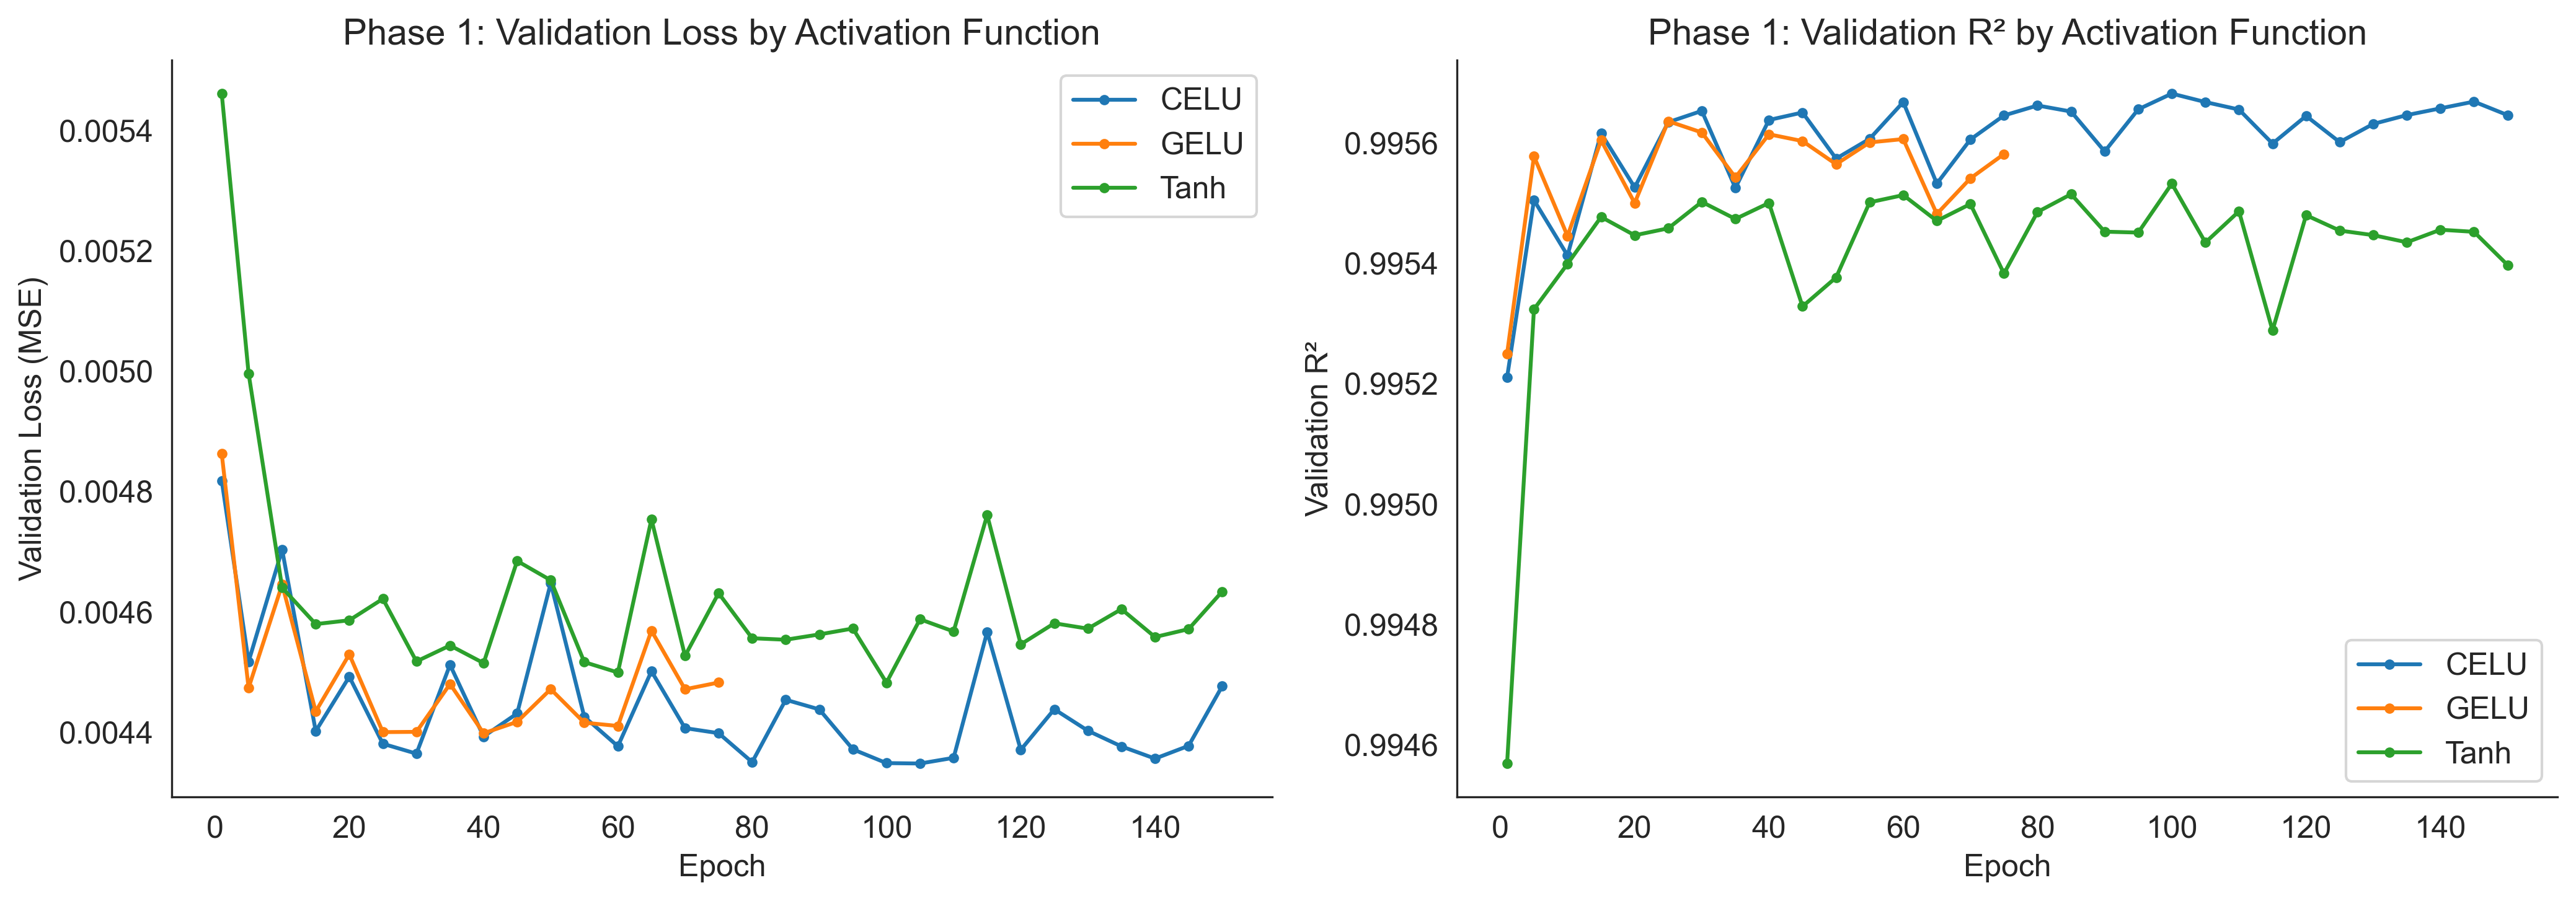
\includegraphics[width=0.95\textwidth]{Thesis/Chapter 4/Figures/fig_phase1_activation_comparison.png}
\caption{Phase~1: validation MSE loss (left) and validation $R^2$
(right) by activation function over training epochs.}
\label{fig:phase1_activation_annex}
\end{figure}

\begin{figure}[H]
\centering
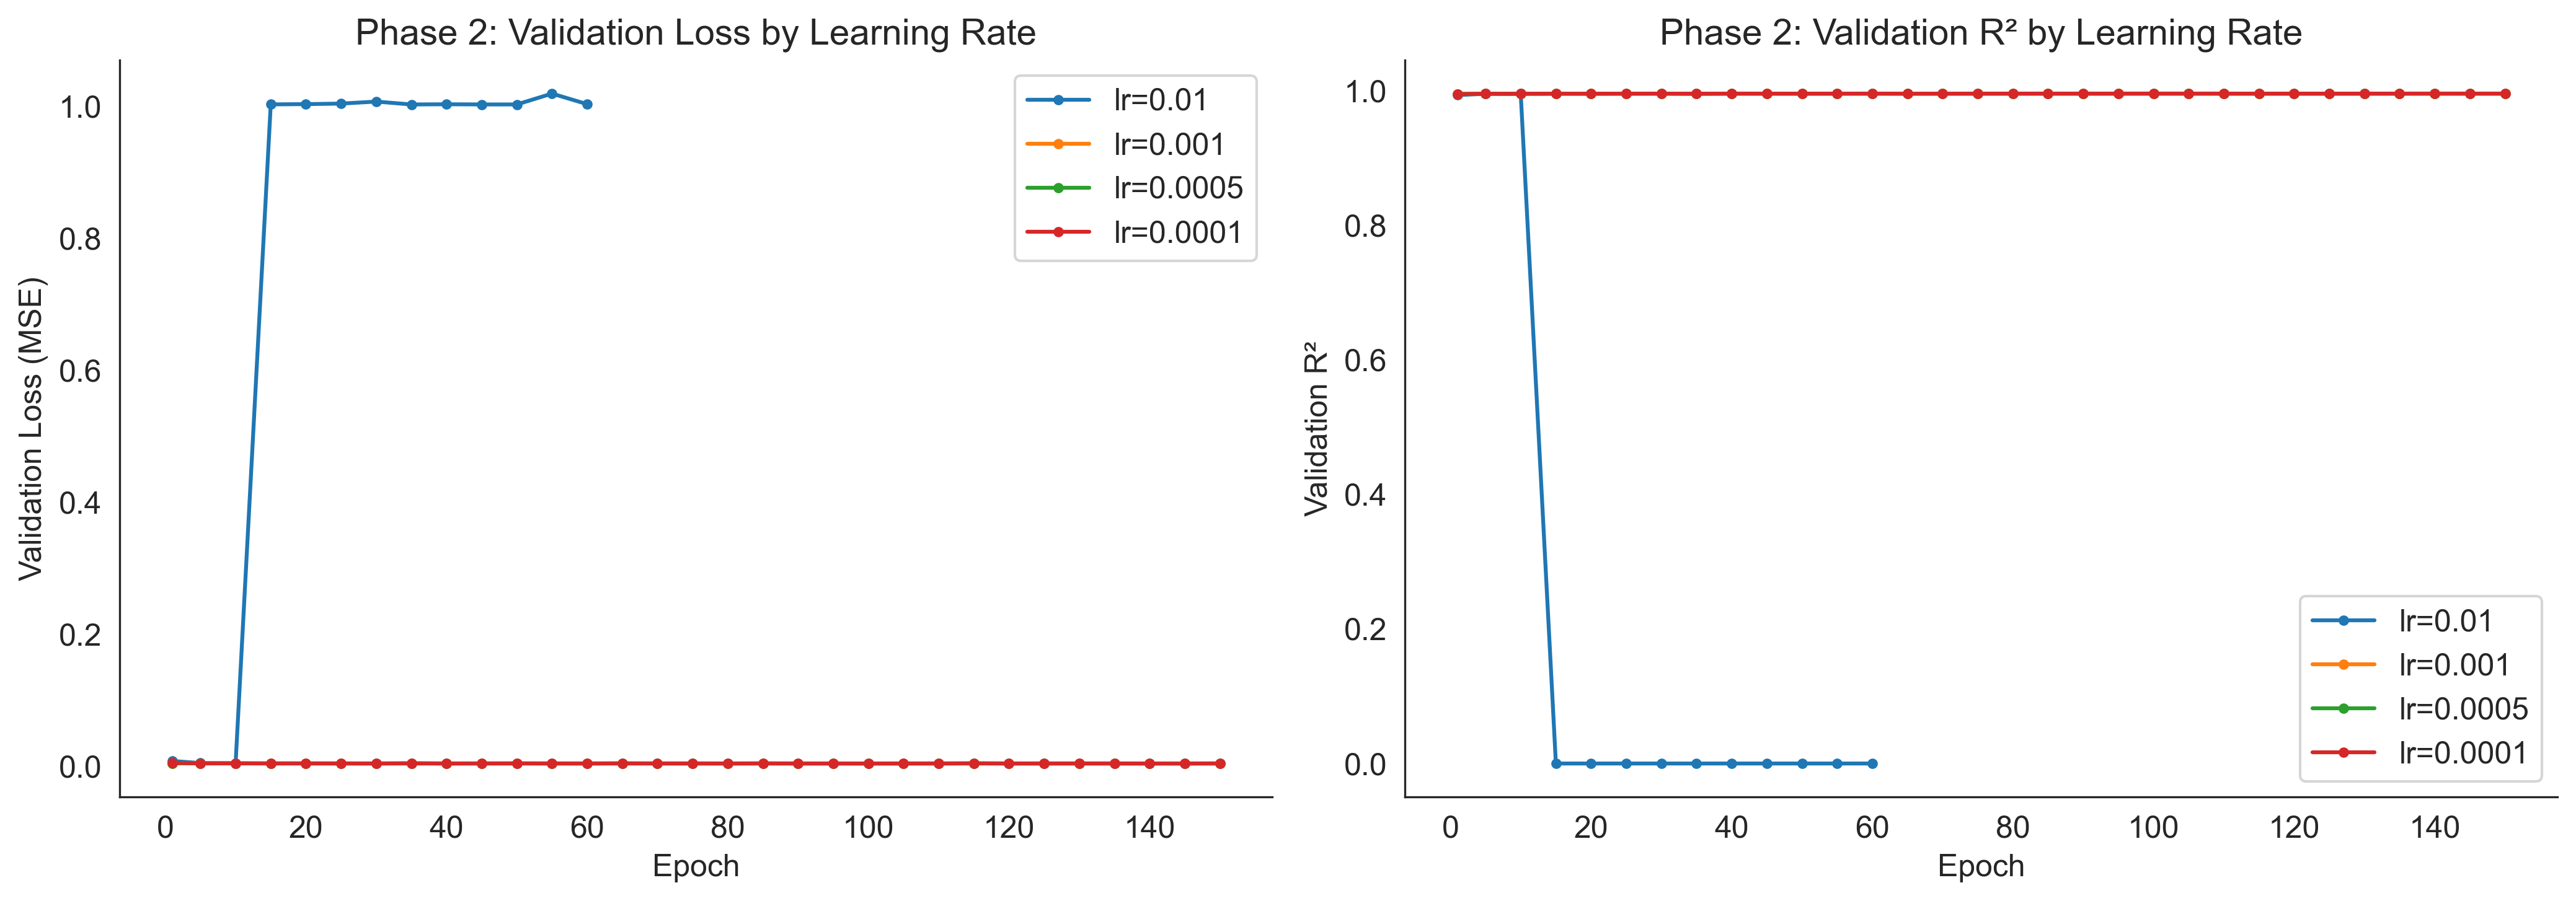
\includegraphics[width=0.95\textwidth]{Thesis/Chapter 4/Figures/fig_phase2_lr_comparison.png}
\caption{Phase~2: validation MSE loss (left) and validation $R^2$
(right) by learning rate.}
\label{fig:phase2_lr_annex}
\end{figure}

\begin{figure}[H]
\centering
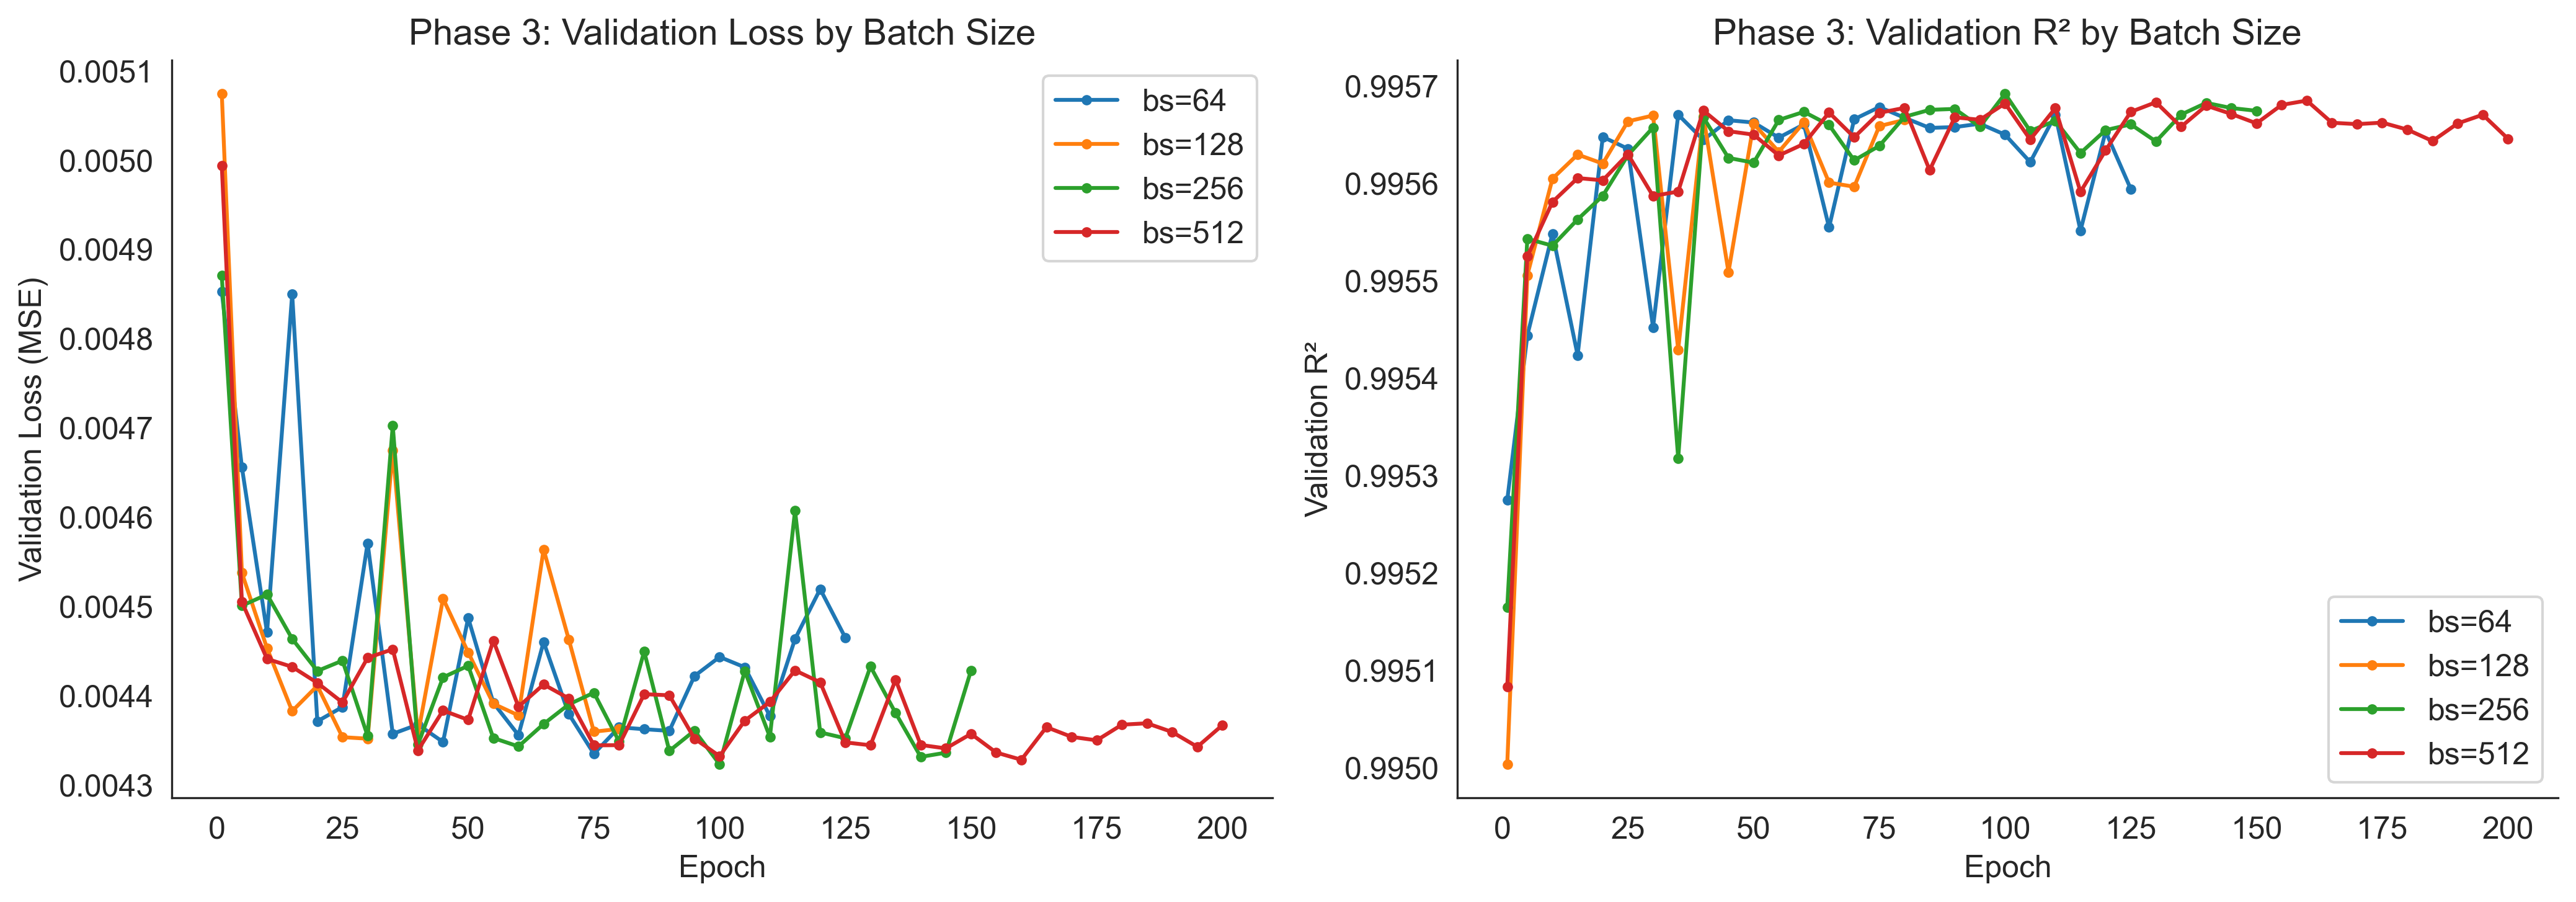
\includegraphics[width=0.95\textwidth]{Thesis/Chapter 4/Figures/fig_phase3_batchsize_comparison.png}
\caption{Phase~3: validation MSE loss (left) and validation $R^2$
(right) by batch size.}
\label{fig:phase3_batchsize_annex}
\end{figure}

\begin{figure}[H]
\centering
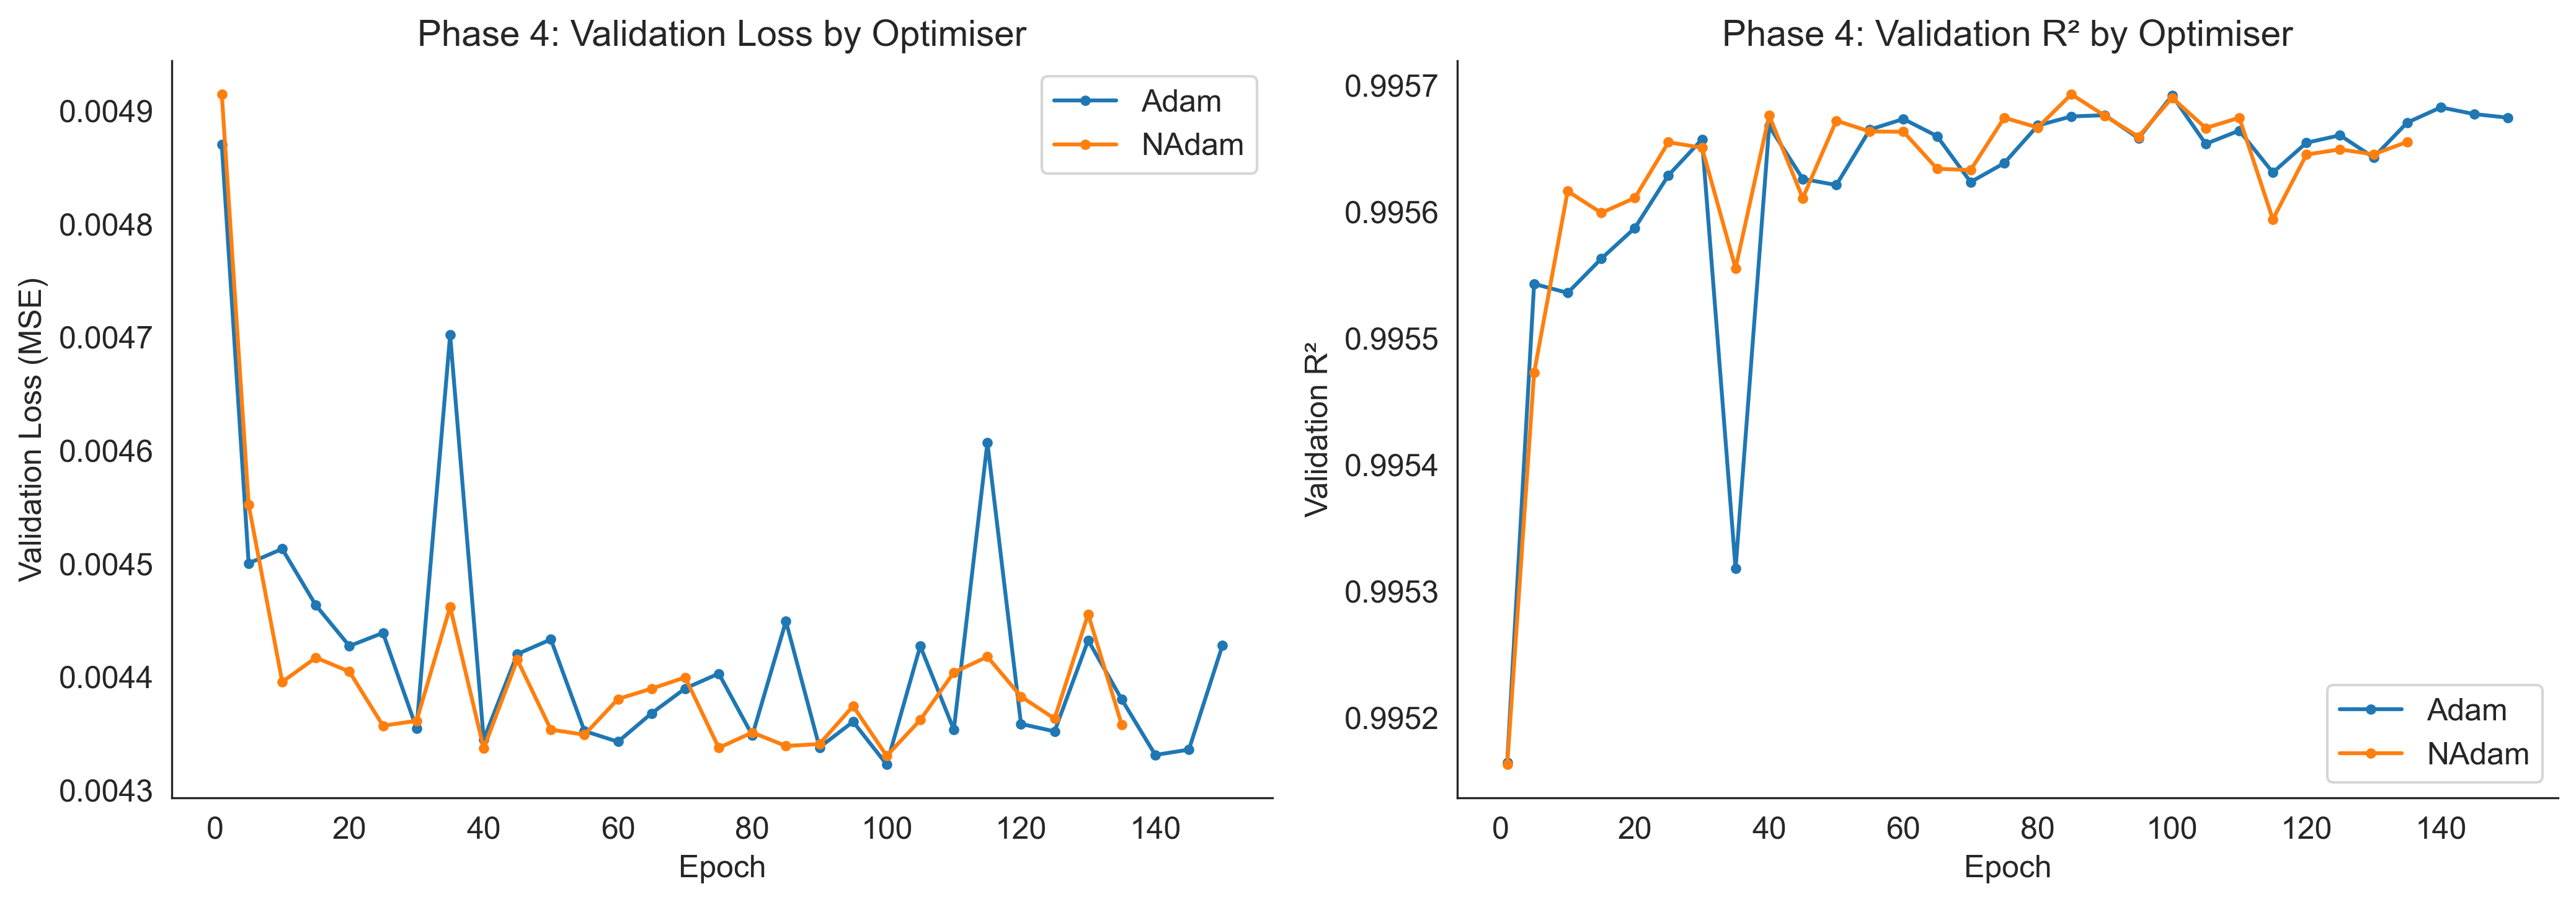
\includegraphics[width=0.95\textwidth]{Thesis/Chapter 4/Figures/fig_phase4_optimiser_comparison.png}
\caption{Phase~4: validation MSE loss (left) and validation $R^2$
(right) by optimiser.}
\label{fig:phase4_optimiser_annex}
\end{figure}

\begin{figure}[H]
\centering
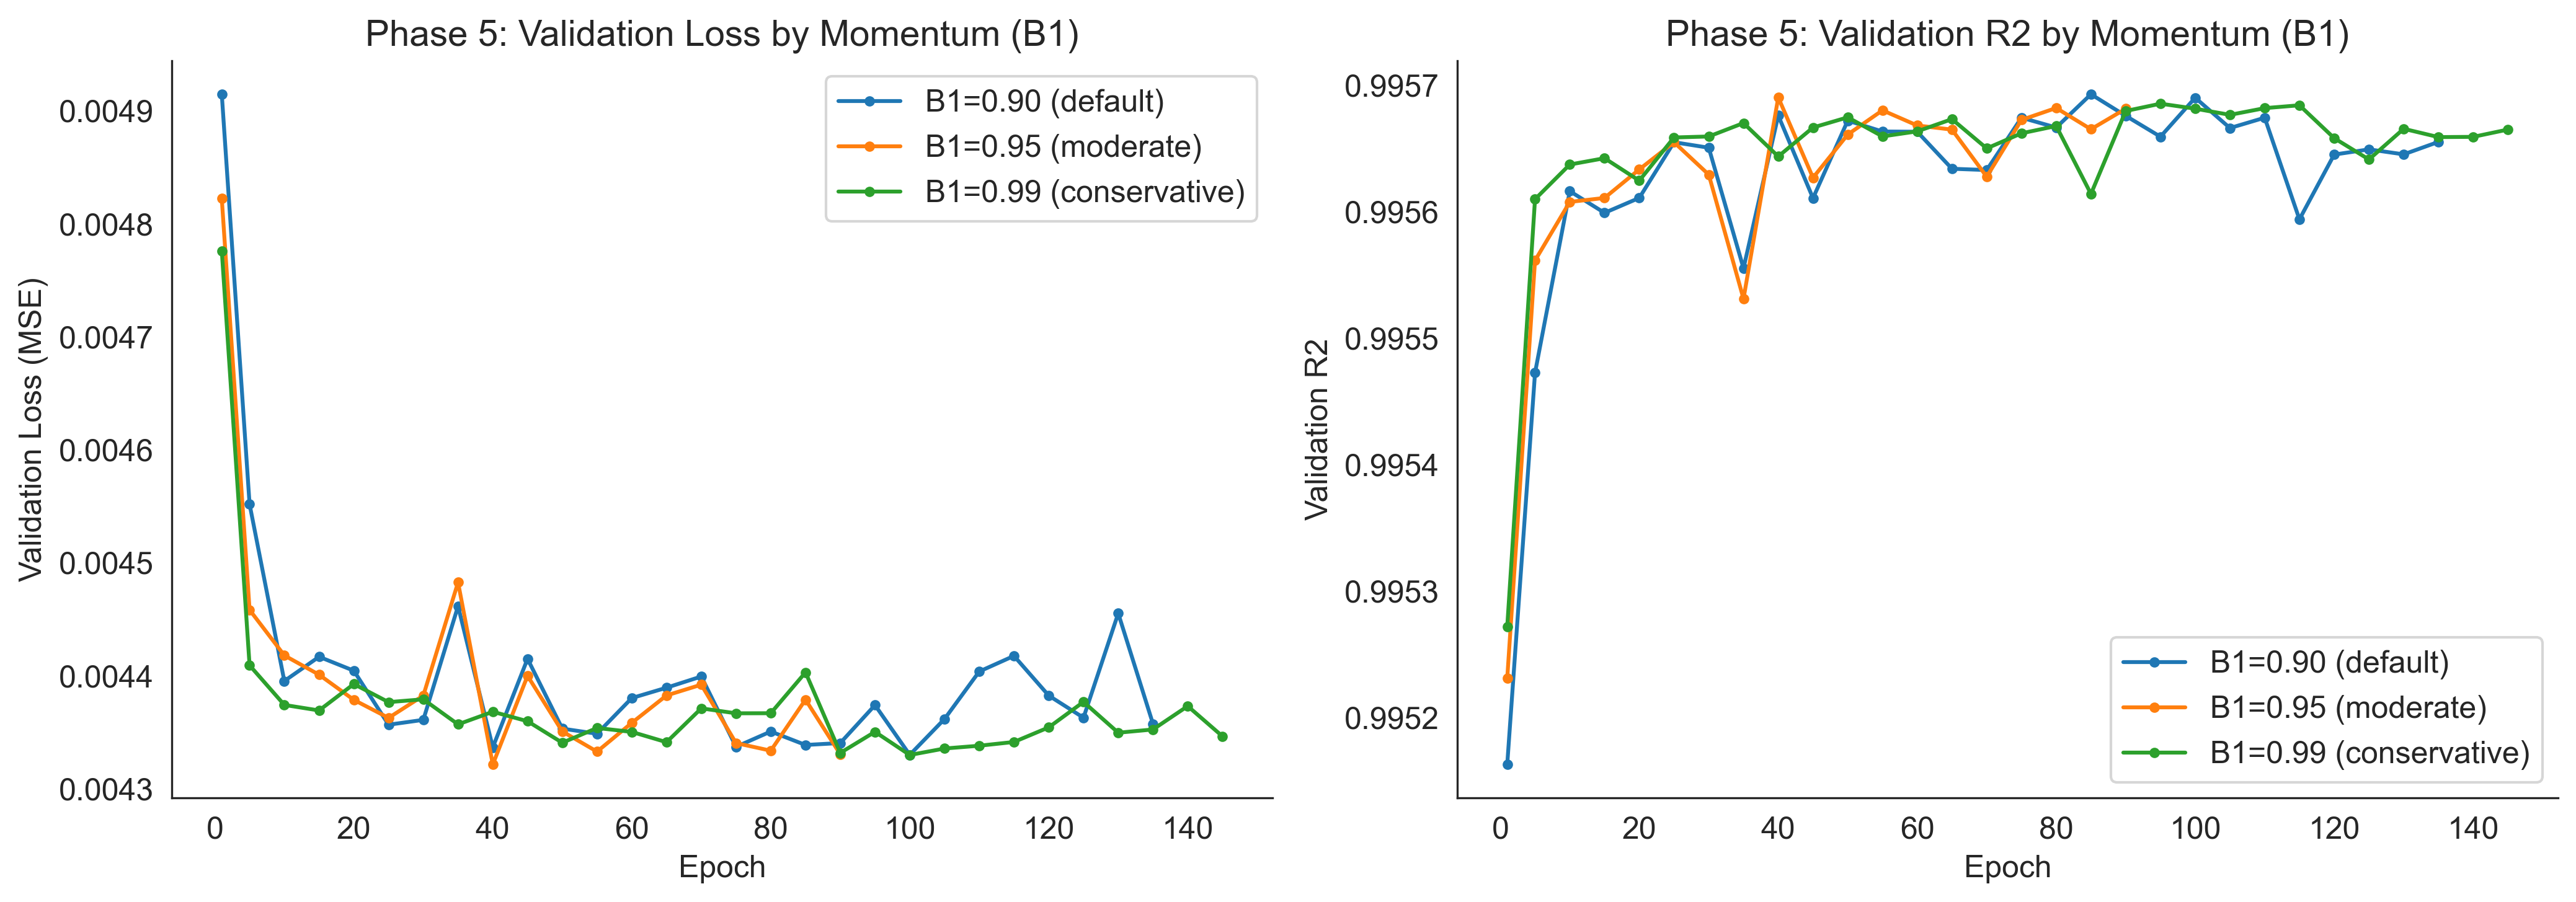
\includegraphics[width=0.95\textwidth]{Thesis/Chapter 4/Figures/fig_phase5_momentum_comparison.png}
\caption{Phase~5: validation MSE loss (left) and validation $R^2$
(right) by first momentum coefficient $\beta_1$.}
\label{fig:phase5_momentum_annex}
\end{figure}

\begin{figure}[H]
\centering
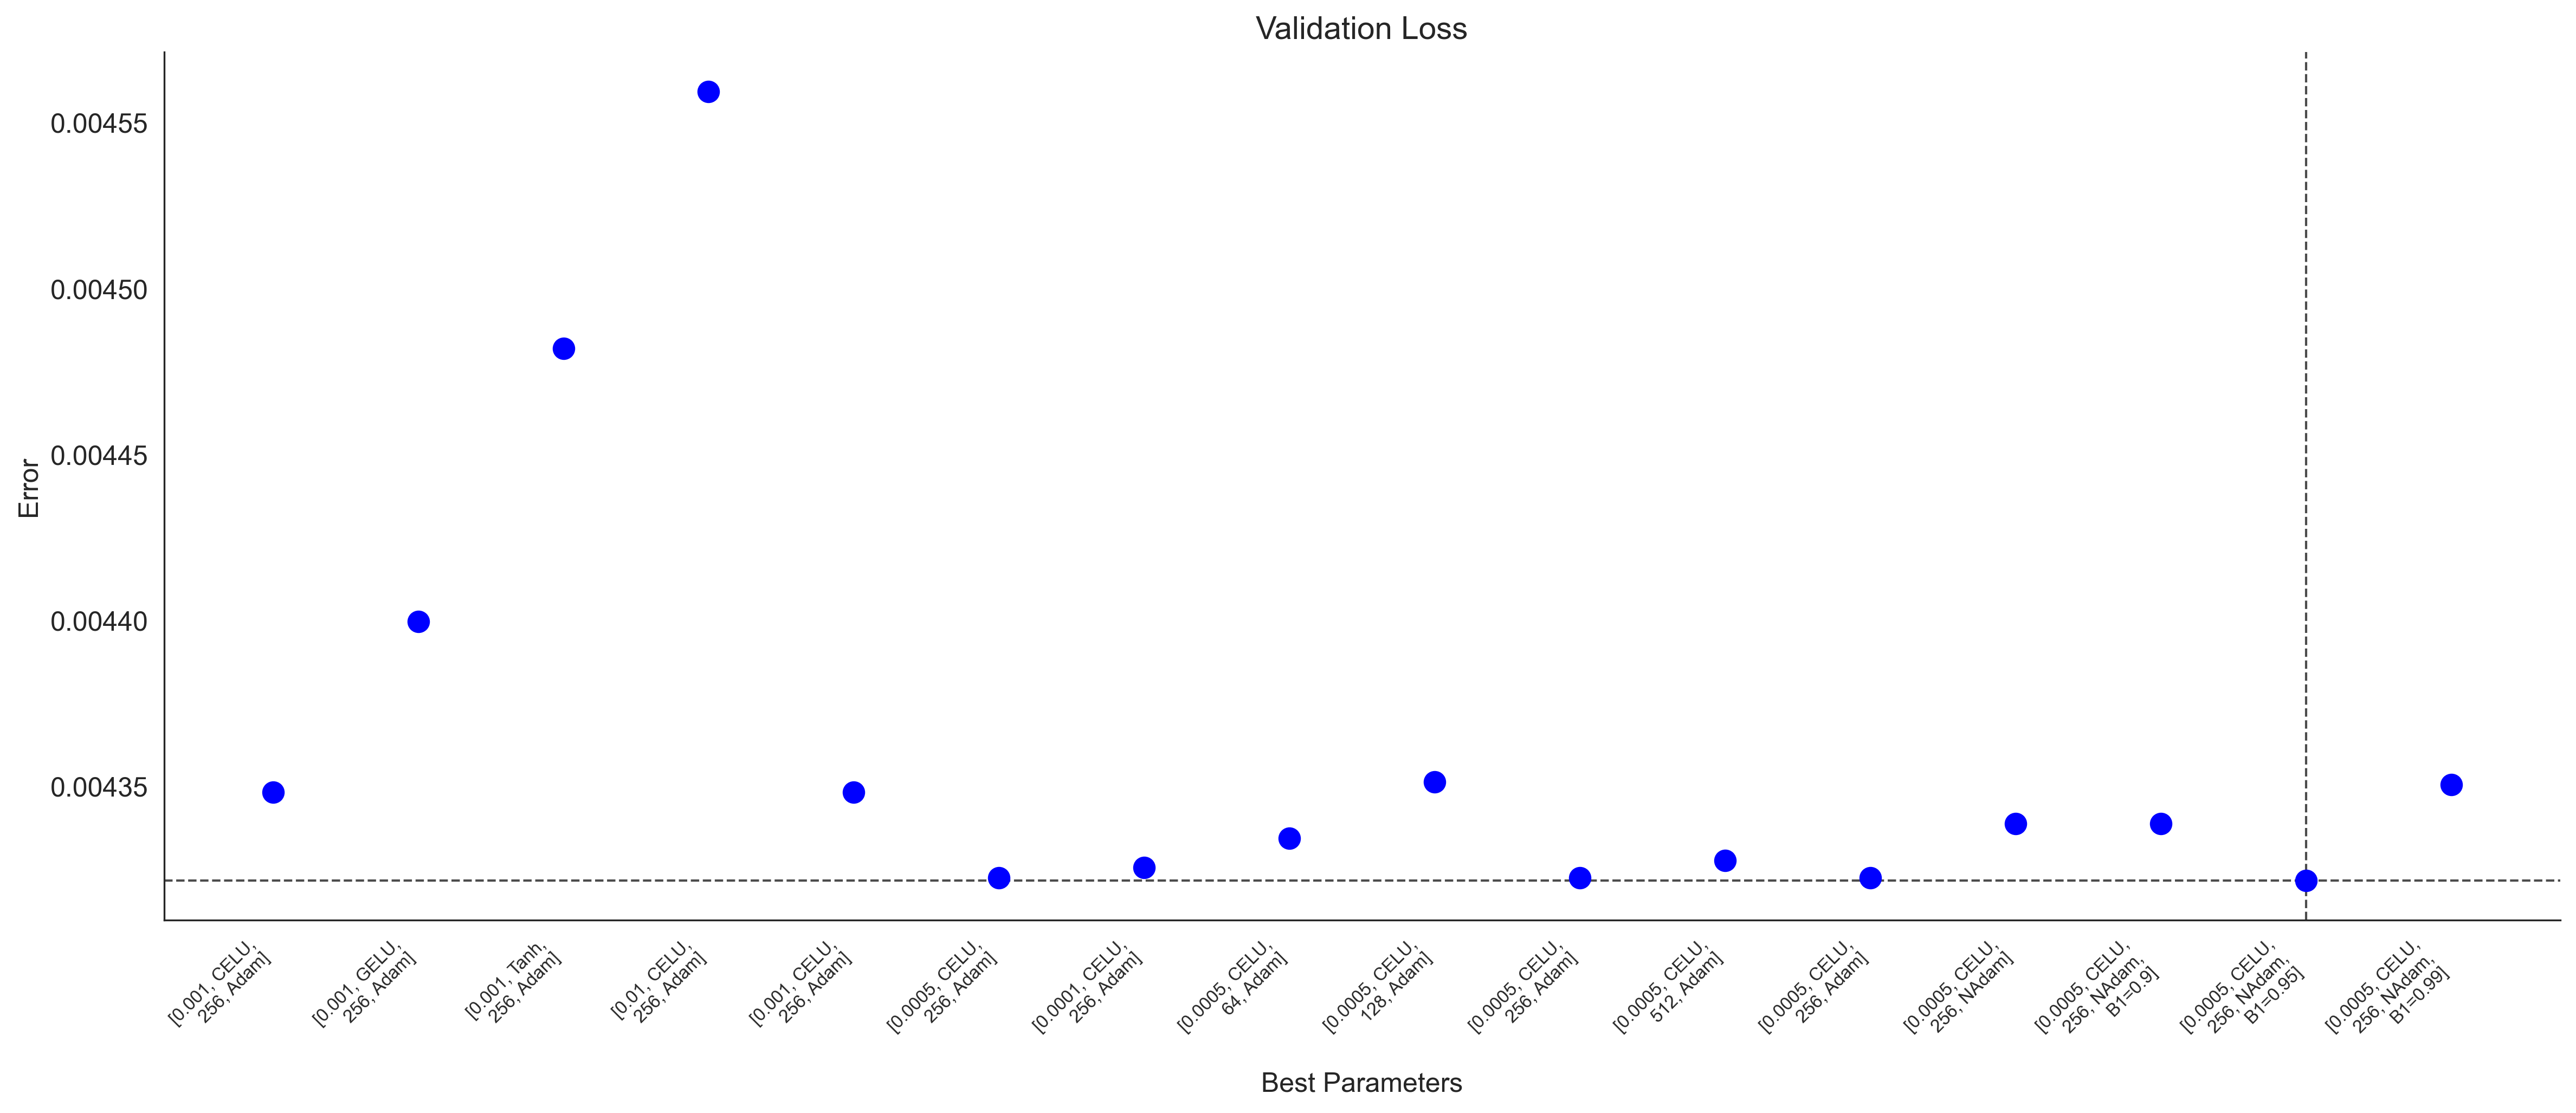
\includegraphics[width=0.95\textwidth]{Thesis/Chapter 4/Figures/fig_validation_loss_hyperparameters.png}
\caption{Best validation MSE loss across all hyperparameter
configurations evaluated in Phases~1 to~5.}
\label{fig:validation_loss_overview_annex}
\end{figure}

% -------------------------------------------------------------
\subsection{Bayesian Optimisation: GP Surrogate}
\label{annexure:bo_methodology}

A Gaussian process surrogate with a Mat\'{e}rn $\nu = 5/2$ kernel was fitted to the observed hyperparameter evaluations to visualise the validation-error landscape. The GP was fitted using scikit-learn's \texttt{GaussianProcessRegressor} with 15 random restarts, seed 42, and a composite kernel consisting of a constant kernel multiplied by the Mat\'{e}rn kernel plus a white noise kernel. Log-scaled axes were used for the learning rate dimension. The fitted surface and its uncertainty were evaluated on a $100 \times 100$ grid with 15\% margin beyond the observed range.

% -------------------------------------------------------------
\subsection{Consolidated Best Hyperparameter Summary}
\label{annexure:best_hyperparams}

\begin{table}[htbp]
\centering
\caption{Best hyperparameter configuration selected for the final DNN model.}
\label{tab:best_hyperparams}
\begin{tabular}{ll}
\toprule
\textbf{Hyperparameter} & \textbf{Selected Value} \\
\midrule
Architecture    & $22 \to 256 \to 128 \to 64 \to 32 \to 16 \to 1$ \\
Activation      & CELU \\
Learning rate   & 0.0005 \\
Batch size      & 256 \\
Optimiser       & NAdam \\
$\beta_1$       & 0.90 \\
$\beta_2$       & 0.999 \\
Bias            & False (all layers) \\
Max epochs      & 100 \\
Early stopping  & 10 checks (every 5 epochs) \\
Loss function   & MSE (on normalised scale) \\
\bottomrule
\end{tabular}
\end{table}

